\subsection{Data preparation}
In this section we focus on describing our new dataset, cleaned and composed by some new features derived by the original ones.

\subsubsection{Building the player's profile}
The purpose of data preparation is building a profile that will be feeded to the clustering analysis, as a starting point we decided to build such profile from the features we had from the matches dataset.

\paragraph{Sex}
First of all, when we started building our new dataset, we assigned the sex to each player inside tennis\_matches using the female\_players and male\_players datasets. Some players of the tennis\_matches dataset were not found in the "sex" dataset due to spelling errors in their name, but we solved this problem by looking online.
\begin{figure}[H]
    \centering
    \subfloat[Sex distribution]{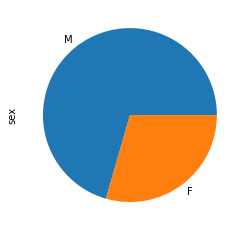
\includegraphics[width=0.20\linewidth]{images/data_preparation/sex_distribution.png}}
    \subfloat[Age distribution]{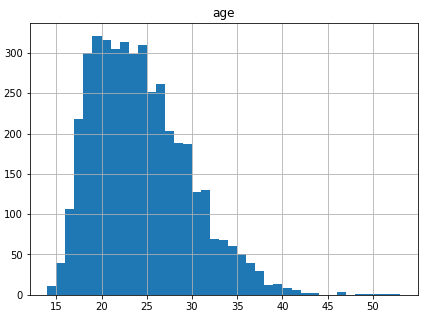
\includegraphics[width=0.32\linewidth]{images/data_preparation/age_distribution.png}}
    \caption{Sex and age distribution}
    \label{fig:sex_age_feature}
\end{figure}
\paragraph{Age}
Since we are doing a "current" analysis, we assign to each one of the players the last age they appear in the original dataset. Some of them have an unknown one, we had to sample it.

\paragraph{Ioc} This was the easiest one since we didn't have to deal with missing values.
\begin{figure}[H]
    \centering
    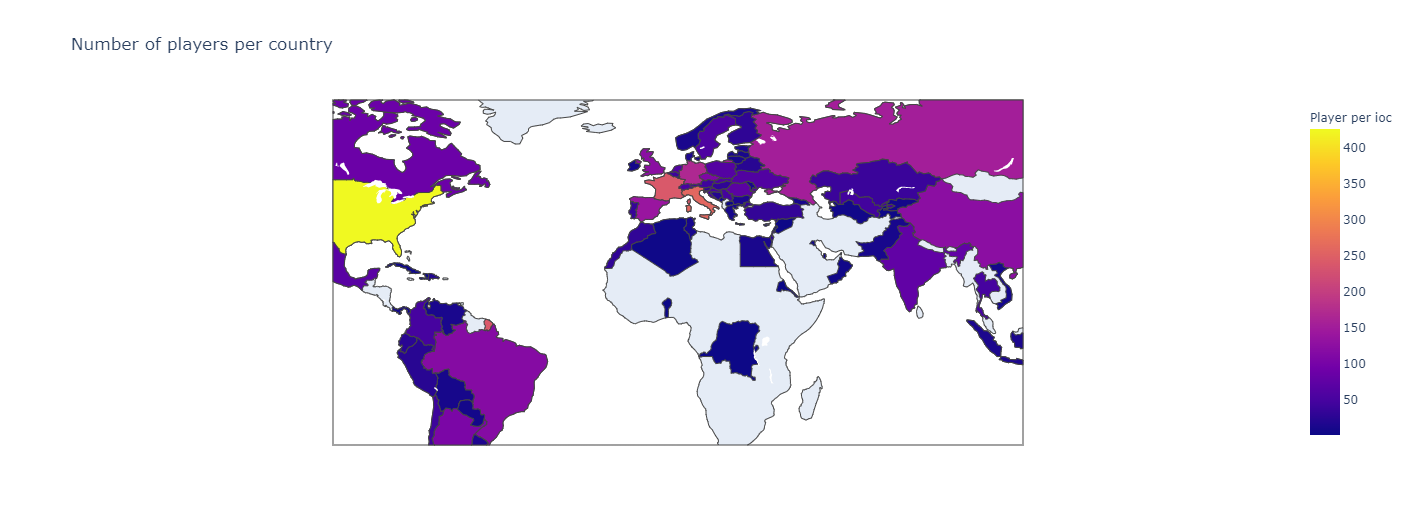
\includegraphics[width=0.74\linewidth]{images/data_preparation/ioc_distribution.png}
    \caption{IOC distribution}
    \label{fig:ioc_feature}
\end{figure}

\paragraph{Height} We solve the issue of having many players without an height, for this purpose we sample their height from the distributions based on countries and sex where this is possible, otherwise we assign them the mean height of their respective sex.

\paragraph{Hand} Just like for the ioc we just needed to assign the hand to the players since the missing values were already dealt with.

\paragraph{Wins and losses} We calculated the total matches won or lost by the player and also how many matches they won on a specific surface.

\paragraph{Tournaments won} We calculated the tournaments won by the player by looking at how many times he appeared in a final as the winner.

\paragraph{Surfaces} We inserted the amount of wins by a player for each surface he/she played on.

\paragraph{Statistics, rank and rank points} For each player we calculated all the statistics coming from the cleaned matches dataset, futhermore we assigned at each player their rank and rank points, eliminating from the dataframe those played less than ten matches.

\subsubsection{Building new features}
Having inserted the feature coming from the cleaned matches dataset it was time to look at the correlation between the features.
\begin{figure}[H]
    \centering
    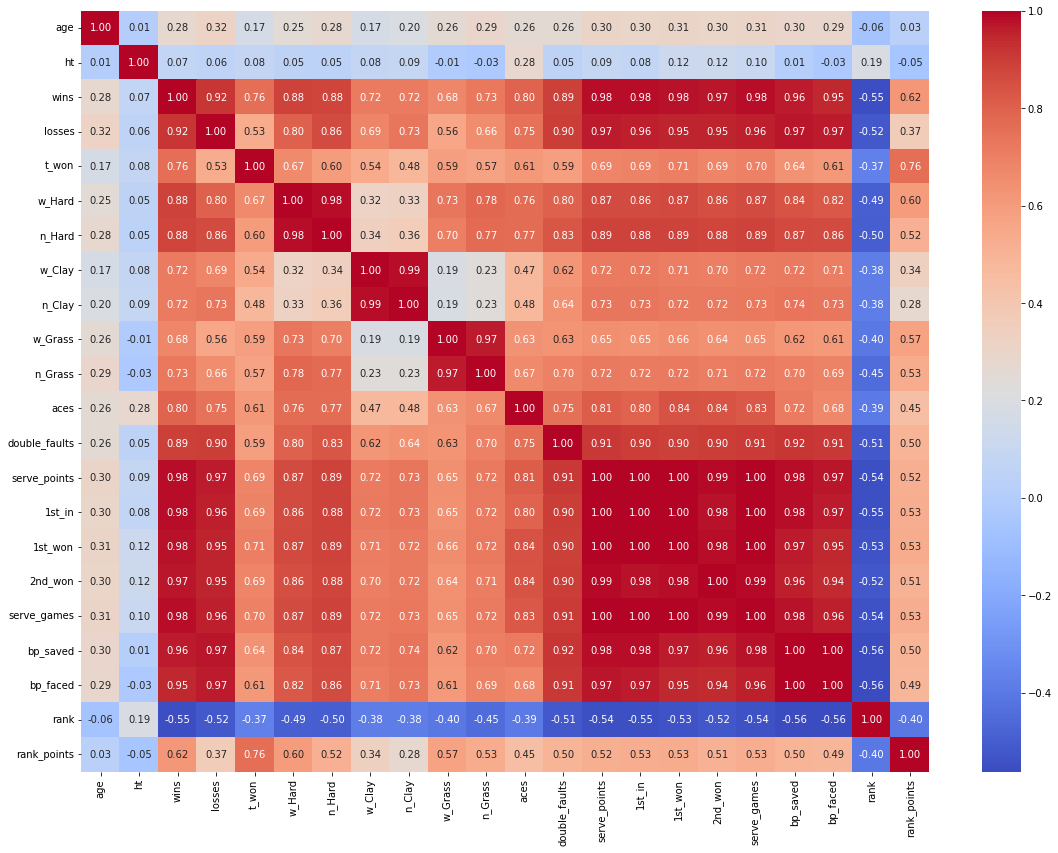
\includegraphics[width= 0.59\linewidth]{images/data_preparation/correlations_before_new_features.png}
    \caption{Correlation matrix of the new dataset with the features coming from the matches dataset.}
    \label{fig:corr_matrix_old_features}
\end{figure}
As we can see from \autoref{fig:corr_matrix_old_features}, there were many highly-correlated feature, so we decided to build new ones from those that we had in the dataframe, such as [\textit{num\_matches, p\_wins, p\_w\_Hard, p\_w\_Clay, p\_w\_Grass, mean\_ace and p\_aces, mean\_double\_faults and p\_double\_faults, mean\_1st\_in and p\_1st\_in, mean\_1st\_won and p\_1st\_won, mean\_2nd\_won and p\_2nd\_won,\\mean\_bp\_saved and p\_bp\_saved, mean\_bp\_faced, mean\_sv\_games, mean\_sv\_points}]

\paragraph{Categorical features} We build categorical attributes that split players by age, height and rank ranges.
\vspace{3mm}

We then dropped the features that were too high correlated with another one or we deemed useless for the players analysis (n\_matches, mean\_aces, mean\_sv\_games, mean\_double\_faults).
After adding the new derived features, we checked that they were not correlated each other by calculating again the correlation matrix, as showed in \autoref{fig:corr_matrix_new_ds}.

\begin{figure}[H]
    \centering
    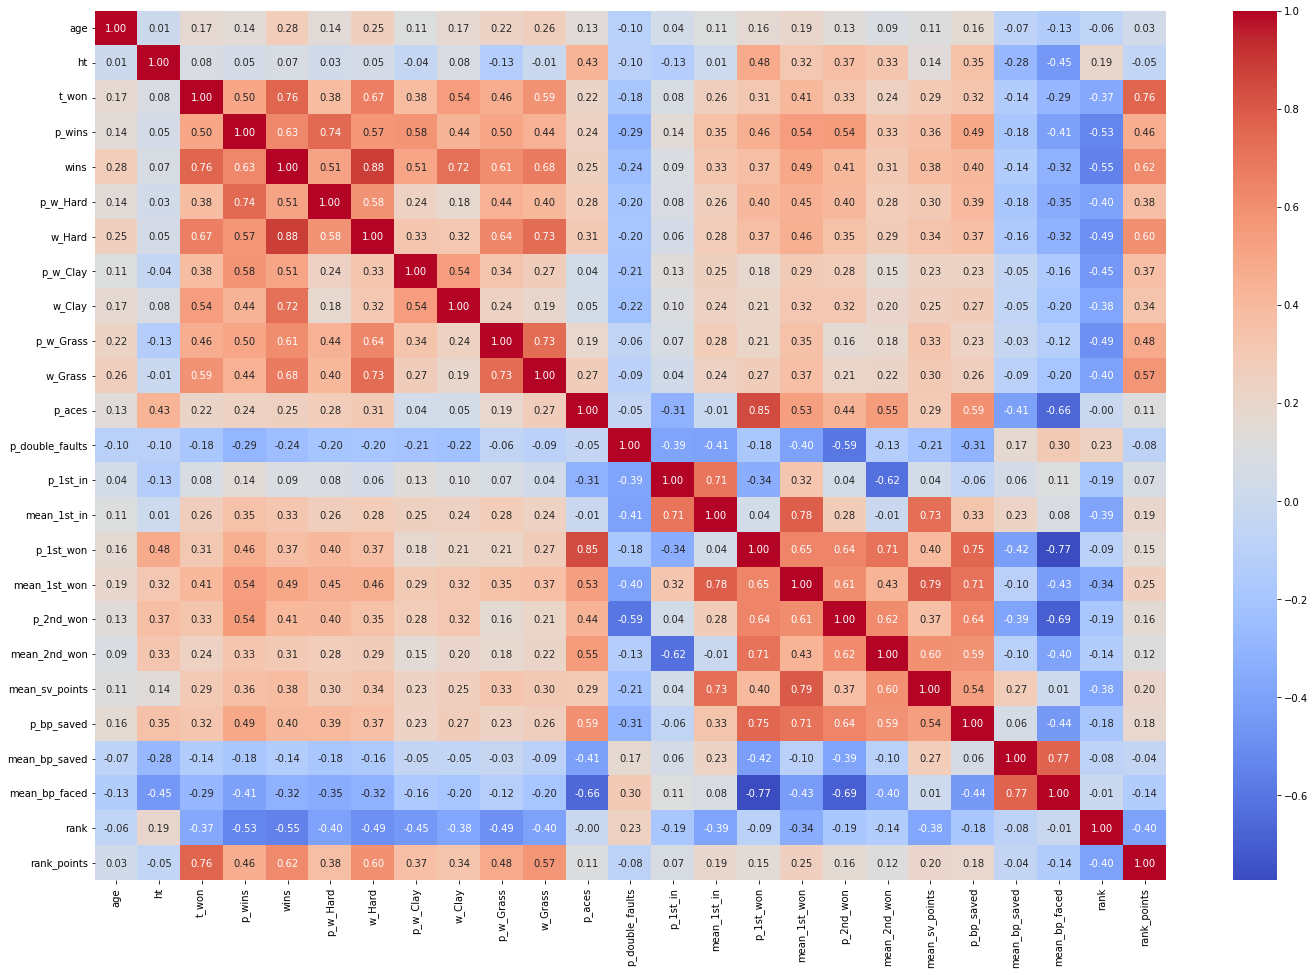
\includegraphics[width=0.7\linewidth]{images/data_preparation/players_corr_features.png}
    \caption{Correlation matrix of the new dataset with the feature we added.}
    \label{fig:corr_matrix_new_ds}
\end{figure}